\chapter{Heaven's reality}

The \emcap{personality of God} deals with the quality or state of God being a person. Whenever we look at the pioneer's work on the \emcap{personality of God}, we see that they were all in harmony with the view that God is a tangible \textit{being}, possessing both body and parts. We always see the same underlying reasoning, which differentiates the term ‘\textit{spirit}’ and the term ‘\textit{being}’. By differentiating these terms, they explain the quality or state of God being a person\footnote{\href{https://www.merriam-webster.com/dictionary/personality}{Merriam-Webster Dictionary} defines the word ‘\textit{personality}’ as “\textit{quality or state of being a person}”.}—a \emcap{personality of God}. All their conclusions are summed up in the first point of the \emcap{Fundamental Principles}. \others{There is \textbf{one God}, a \textbf{personal}, \textbf{spiritual being}, the Creator of all things, omnipotent, omniscient, … and \textbf{every-where present by his representative, the Holy Spirit}. Psalm 139:7.}[FPSDA 1.2][https://egwwritings.org/read?panels=p1299.6]

So far, in the pioneers’ work, we have seen that the \emcap{personality of God} is tightly connected to the reality of God’s presence. God is a personal spiritual being, having a body and shape; as such, His presence is cumbered to one locality—as the Bible says, in His temple, at His throne where He is surrounded with unapproachable glory. But He is everywhere present by His representative, the Holy Spirit. Obviously, the Holy Spirit is a spirit, and not a being, \bible{for a spirit hath not flesh and bones as ye see me have}, said Jesus (Luke 24:39). Christ is also a Being, like His Father. He is an express image of the Father’s person; therefore, He bears the same personality, or the quality or state of being a person, as His Father does.

In our experience, when we present the original Seventh-day Adventist beliefs on the \emcap{personality of God} to our trinitarian brothers, as expressed in the first two points of the \emcap{Fundamental Principles}, they often claim that the statements in the \emcap{Fundamental Principles} are correct in some way, but the understanding attributed to the terms “\textit{personal spiritual being}” are false. They usually attempt to harmonize the \emcap{Fundamental Principles} with the Trinity doctrine by twisting the words “\textit{spiritual being}”, as if the word ‘\textit{spiritual}’ means something mysterious, suitable to equalize the \emcap{personality of God} and of Christ with the personality of the Holy Ghost\footnote{The quality or state of the Holy Spirit being a person is bearing witness, not having the form of a person. \egw{\textbf{The Holy Spirit has a personality}, \textbf{\underline{else} He could not \underline{bear witness} to our spirits} and with our spirits that we are the children of God. \textbf{He must also be a divine person}, \textbf{\underline{else} He could not \underline{search out} the secrets which lie hidden in the mind of God}. ‘For what man knoweth the things of a man save the spirit of man, which is in him; even so the things of God knoweth no man, but the Spirit of God.’ [1 Corinthians 2:11.]}[21LtMs, Ms 20, 1906, par. 32][https://egwwritings.org/read?panels=p14071.10296041&index=0]. It is crystal clear that the Holy Spirit is a person, yet not in the same way as the Father and the Son, as the Holy Spirit does not possess the quality of an outward physical personage like the Father and the Son do.}. The underlying problem comes down to the understanding of the heavenly realities. The Bible is not silent about heaven, and its realities, and our pioneers understood it well. Below we read about the explanation of the terms “\textit{spiritual being}” from James White and Uriah Smith in their book, “\textit{The Biblical Institute}”. The Bible explains these terms using the example of angels, which are “\textit{spiritual beings}”.

\begin{figure}[hp]
    \centering
    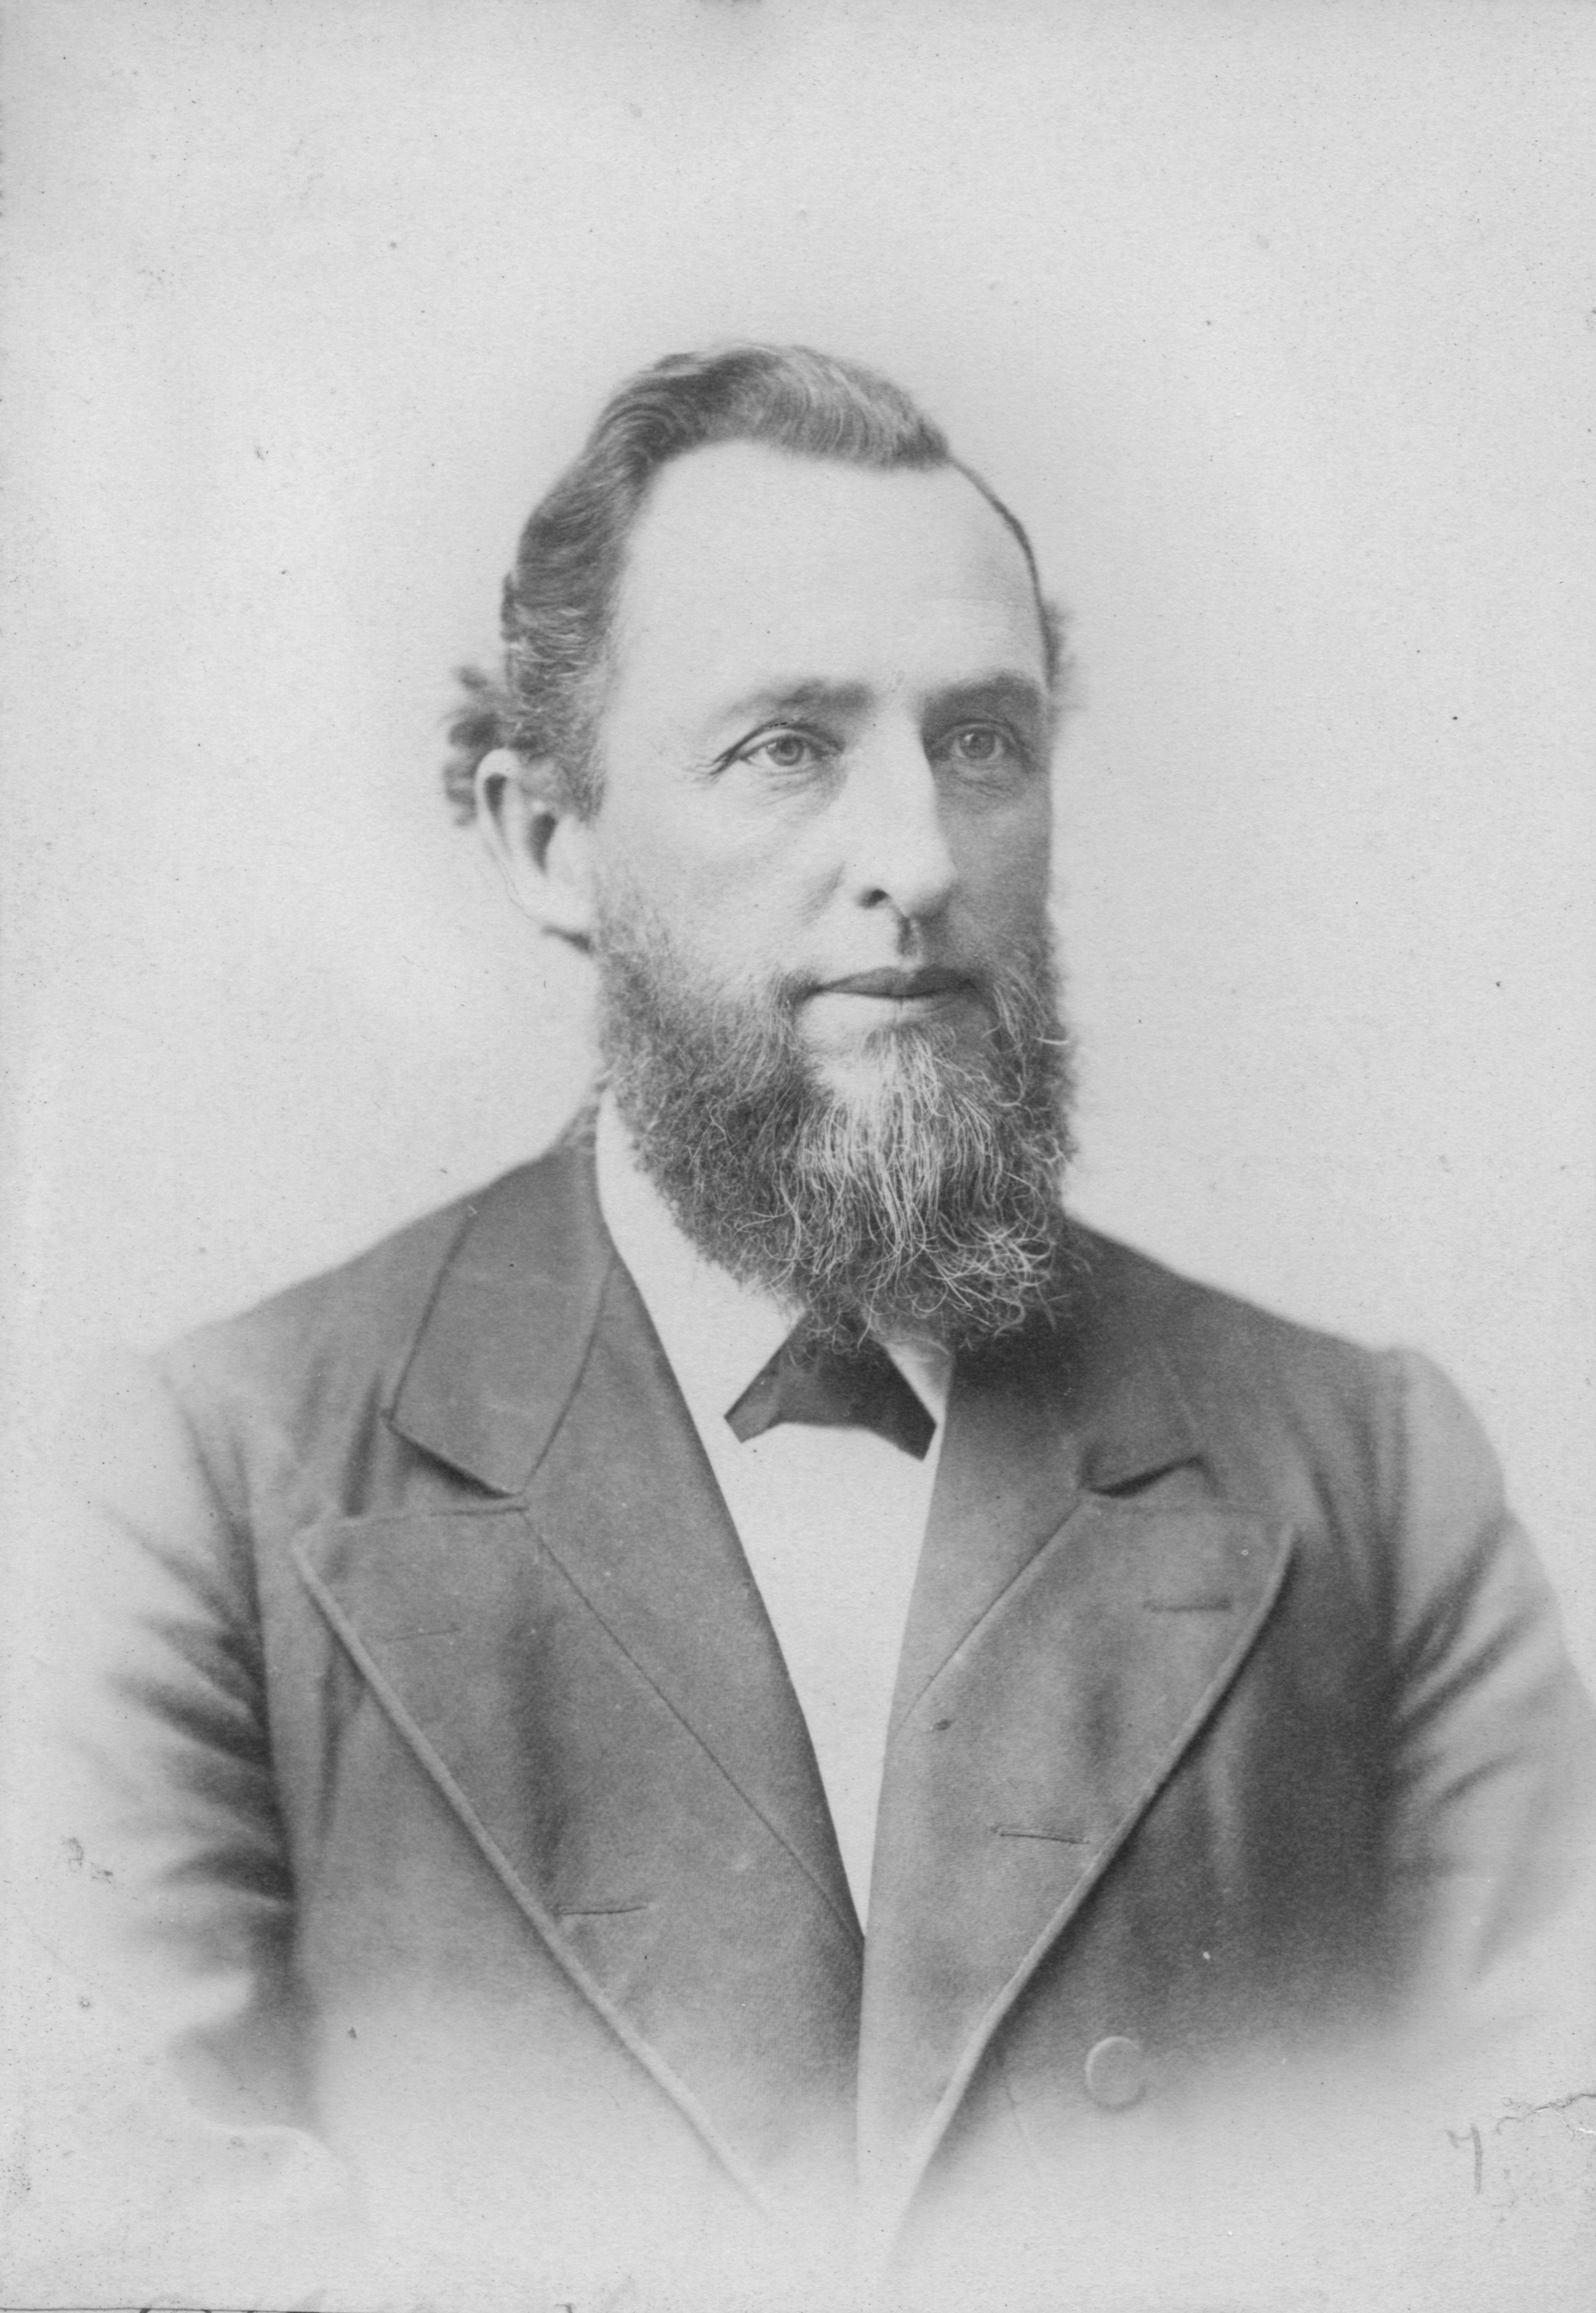
\includegraphics[width=1\linewidth]{images/uriah-smith.jpg}
    \caption*{Uriah Smith (1832-1903)}
    \label{fig:uriah-smith}
\end{figure}

\others{\textbf{Angels are real beings}. They are described in the Bible as \textbf{possessing face, feet, wings} \&x. Ezekiel says of the cherubim, ‘\textbf{Their whole \underline{body} and their backs and their hands and their wings},’ \&c. Eze. 10:12. Angels \textbf{appeared }unto Abraham. Gen. 18:1-8. They talked and ate with him. They went on to Sodom and communed with Lot, who, entering into his house baked unleavened bread for them and they did eat. \textbf{These person were called angels}. David speaks of the manna as the corn of Heaven and angel’s food. Ps. 78:23-25.}

\othersnogap{The case of Balaam, Num. 22:22-31, is an interesting incident. The angel \textbf{appeared }to Balaam with a sword \textbf{drawn in his hand}. The question is sometimes asked \textbf{how angels can be \underline{material beings since we cannot see them}. This case illustrates it}. The record says the \textbf{Lord opened the eyes of Balaam and he saw the angel}. \textbf{The angel did not create a body for that occasion}.\textbf{ He was just the same as he was before Balaam saw him; \underline{but the change took place in Balaam}. His eyes were opened, then he beheld the angel}. It was the same with the servant of Elisha when he and his master were brought into a straight place, surrounded by the army of the king of Syria. 2 Kings 6:17. Elisha prayed that \textbf{the eyes of his servant might be opened}; and he immediately saw the whole mountain full of horses and chariots round about Elisha.}

\othersnogap{\textbf{This may be further illustrated referring to things which we know are material and yet which we cannot see}. Air is material, light is material, even thought itself is only the result of material organizations — matter acting upon matter — and yet we can see none of these things. \textbf{Just so with the angels}.}

\othersnogap{\textbf{It is further objected to the materiality of the angels that they are called spirits. }Heb. 1:13, 14.\textbf{\underline{But this is no objection to their being literal beings}}. \textbf{They are simply spiritual beings organized differently from these earthly bodies which we possess}. Paul says, 1 Cor. 15:44, ‘\textbf{There is a natural body and there is \underline{a spiritual body}}.’ \textbf{The natural body we now have; the spiritual body we shall have in the resurrection}. ‘\textbf{It is raised a spiritual body}.’ Verse 44. \textbf{But then we are equal unto the angels}, Luke 20:36; \textbf{then we have bodies like unto Christ’s most glorious body}. Phil. 3:4\footnote{Typo: It should be Philippians 3:21} \textbf{and Christ is no less a spirit than the angels}. \textbf{We read that God is a spirit, that is, simply \underline{a spiritual being}}.}[James White and Uriah Smith, The Biblical Institute (Kindle Locations 2537-2553). Kindle Edition.]

The Bible gives us the insight that angels are spiritual beings that possess material bodies, but are still unseen to us, unless the Lord opens our eyes to see them. When the righteous will rise up in their new glorified bodies, they will rise in a spiritual body, an incorruptible one. This body will be tangible and material just as the new Earth will be tangible and material. And with our spiritual bodies we will possess the renewed Earth, we will replenish it \bible{and subdue it: and have dominion over the fish of the sea, and over the fowl of the air, and over every living thing that moveth upon the earth}[Genesis 1:28].

% Heaven's reality

\begin{titledpoem}
    
    \stanza{
        God is not vapor, nor mystery unknown, \\
        A personal being upon Heaven's throne. \\
        Bound by space as a being must, \\
        Yet present through His Spirit's trust.
    }

    \stanza{
        Christ bears His image, a tangible Son, \\
        Two divine beings, not mystically one. \\
        Angels around them with bodies unseen, \\
        Material creatures of heavenly sheen.
    }

    \stanza{
        Our eyes cannot witness their spiritual frame, \\
        Until God reveals what our vision can't claim. \\
        In resurrection we'll rise like them too, \\
        Spiritual bodies, yet tangible and true.
    }

    \stanza{
        Not three equal persons in mystical blend, \\
        But Father and Son with Spirit they send. \\
        The divine is not distant, abstract, or obscure, \\
        But personal, present, and perfectly sure.
    }
    
\end{titledpoem}